% Overlap of relevant items found in the top 10 by dense search, BM25 and LightRAG (mix), extended labels.
\begin{figure}[htbp]
\centering
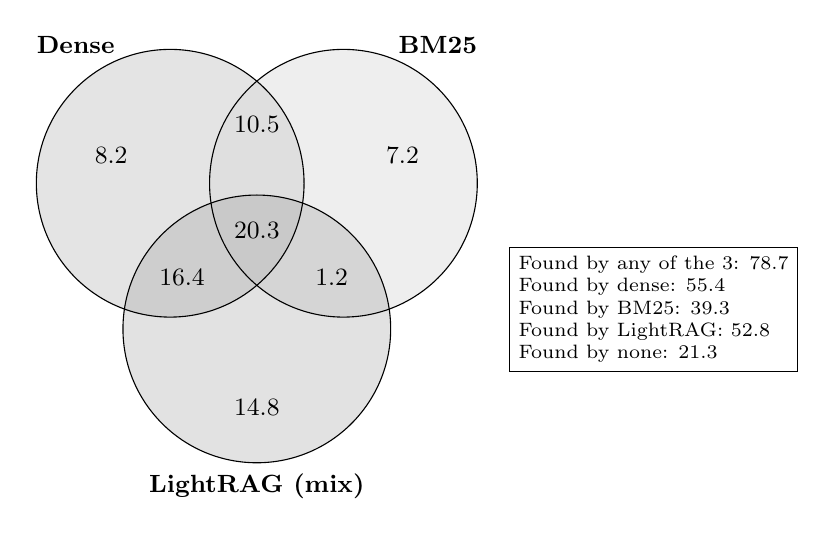
\begin{tikzpicture}[font=\small]
  \fill[black!30,opacity=.35] (0,0) circle (1.7);
  \fill[black!15,opacity=.45] (2.2,0) circle (1.7);
  \fill[black!45,opacity=.25] (1.1,-1.85) circle (1.7);
  \draw (0,0) circle (1.7);
  \draw (2.2,0) circle (1.7);
  \draw (1.1,-1.85) circle (1.7);
  \node[font=\small\bfseries] at (-1.2,1.75) {Dense};
  \node[font=\small\bfseries] at (3.4,1.75) {BM25};
  \node[font=\small\bfseries] at (1.1,-3.85) {LightRAG (mix)};
  \node at (-0.75,0.35) {8.2};
  \node at (2.95,0.35) {7.2};
  \node at (1.1,-2.85) {14.8};
  \node at (1.1,0.75) {10.5};
  \node at (0.15,-1.2) {16.4};
  \node at (2.05,-1.2) {1.2};
  \node at (1.1,-0.6) {20.3};
  \node[draw,align=left,font=\scriptsize,fill=white,anchor=west] at (4.3,-1.6) {Found by any of the 3: 78.7\\Found by dense: 55.4\\Found by BM25: 39.3\\Found by LightRAG: 52.8\\Found by none: 21.3};
\end{tikzpicture}
\caption[Which retrieval method finds which relevant items]{Which retrieval method finds which relevant items on holdout 3. Each region gives the percentage of all 817 relevant items (extended labels, Section~\ref{sec:live-lightrag}) that appear in the top 10 of exactly those methods. The region found only by LightRAG is an upper bound, because LightRAG's results were judged down to rank 10 and those of the other methods mostly to rank 3.}
\label{fig:retrieval-overlap}
\end{figure}
